\section{Results}
We have tested our system comprising 6 slave nodes against a centralized
system making no RPCs. The distributed system was found to take noticeably
longer to handle a batch of bitmap queries of any given size ($0\leq q\leq 1200,$ where $q$ is the number of queries) than the centralized one. The graph below shows that the distributed
system required time $t_d(q)=0.0045q+0.07$ with $R^2=0.9919$ while the centralized system followed the line
$t_c(q)=0.0002q-0.0023$ with $R^2=0.9818$. Since the slope of $t_d(q)$ surpasses the slope of
$t_c(q)$ we expect the distributed system to perform much more slowly. This is due to
the time required to perform RPCs and execute the query planner. Despite the worse performance,
using a distributed system
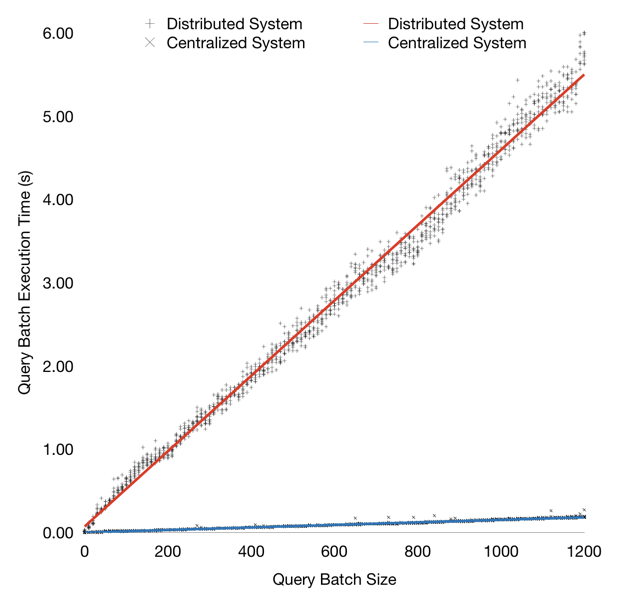
\includegraphics[scale=0.25]{query-experiment-results}
